\section[Conclusiones]{Conclusiones}

	\begin{frame}[plain]
	\frametitle{Conclusión} 
	
	\begin{exampleblock}{Mejora}
		Hemos podido comprobar de primera mano que un cambio en en la optimización o en las prestaciones de la computadora donde se ejecute nuestro algoritmo hace variar las constantes multiplicativas. \\
		Estos cambios pueden ser sustanciales, pero un cambio de algoritmo puede variar la el orden de eficiencia, lo que nos lleva a un cambio mucho más drástico que el que nos proporcionan las constantes ocultas. \\
		Conclusión: mejorar el algoritmo es mejor que mejorar las prestaciones de nuestro ordenador.
	\end{exampleblock}

\end{frame}	
	
	\begin{frame}[plain]
	\frametitle{Tabla Optimizacion 0}
		\begin{figure}[htb]
		\begin{center}
		\begin{picture}(160,0)
		\put(-80,-100){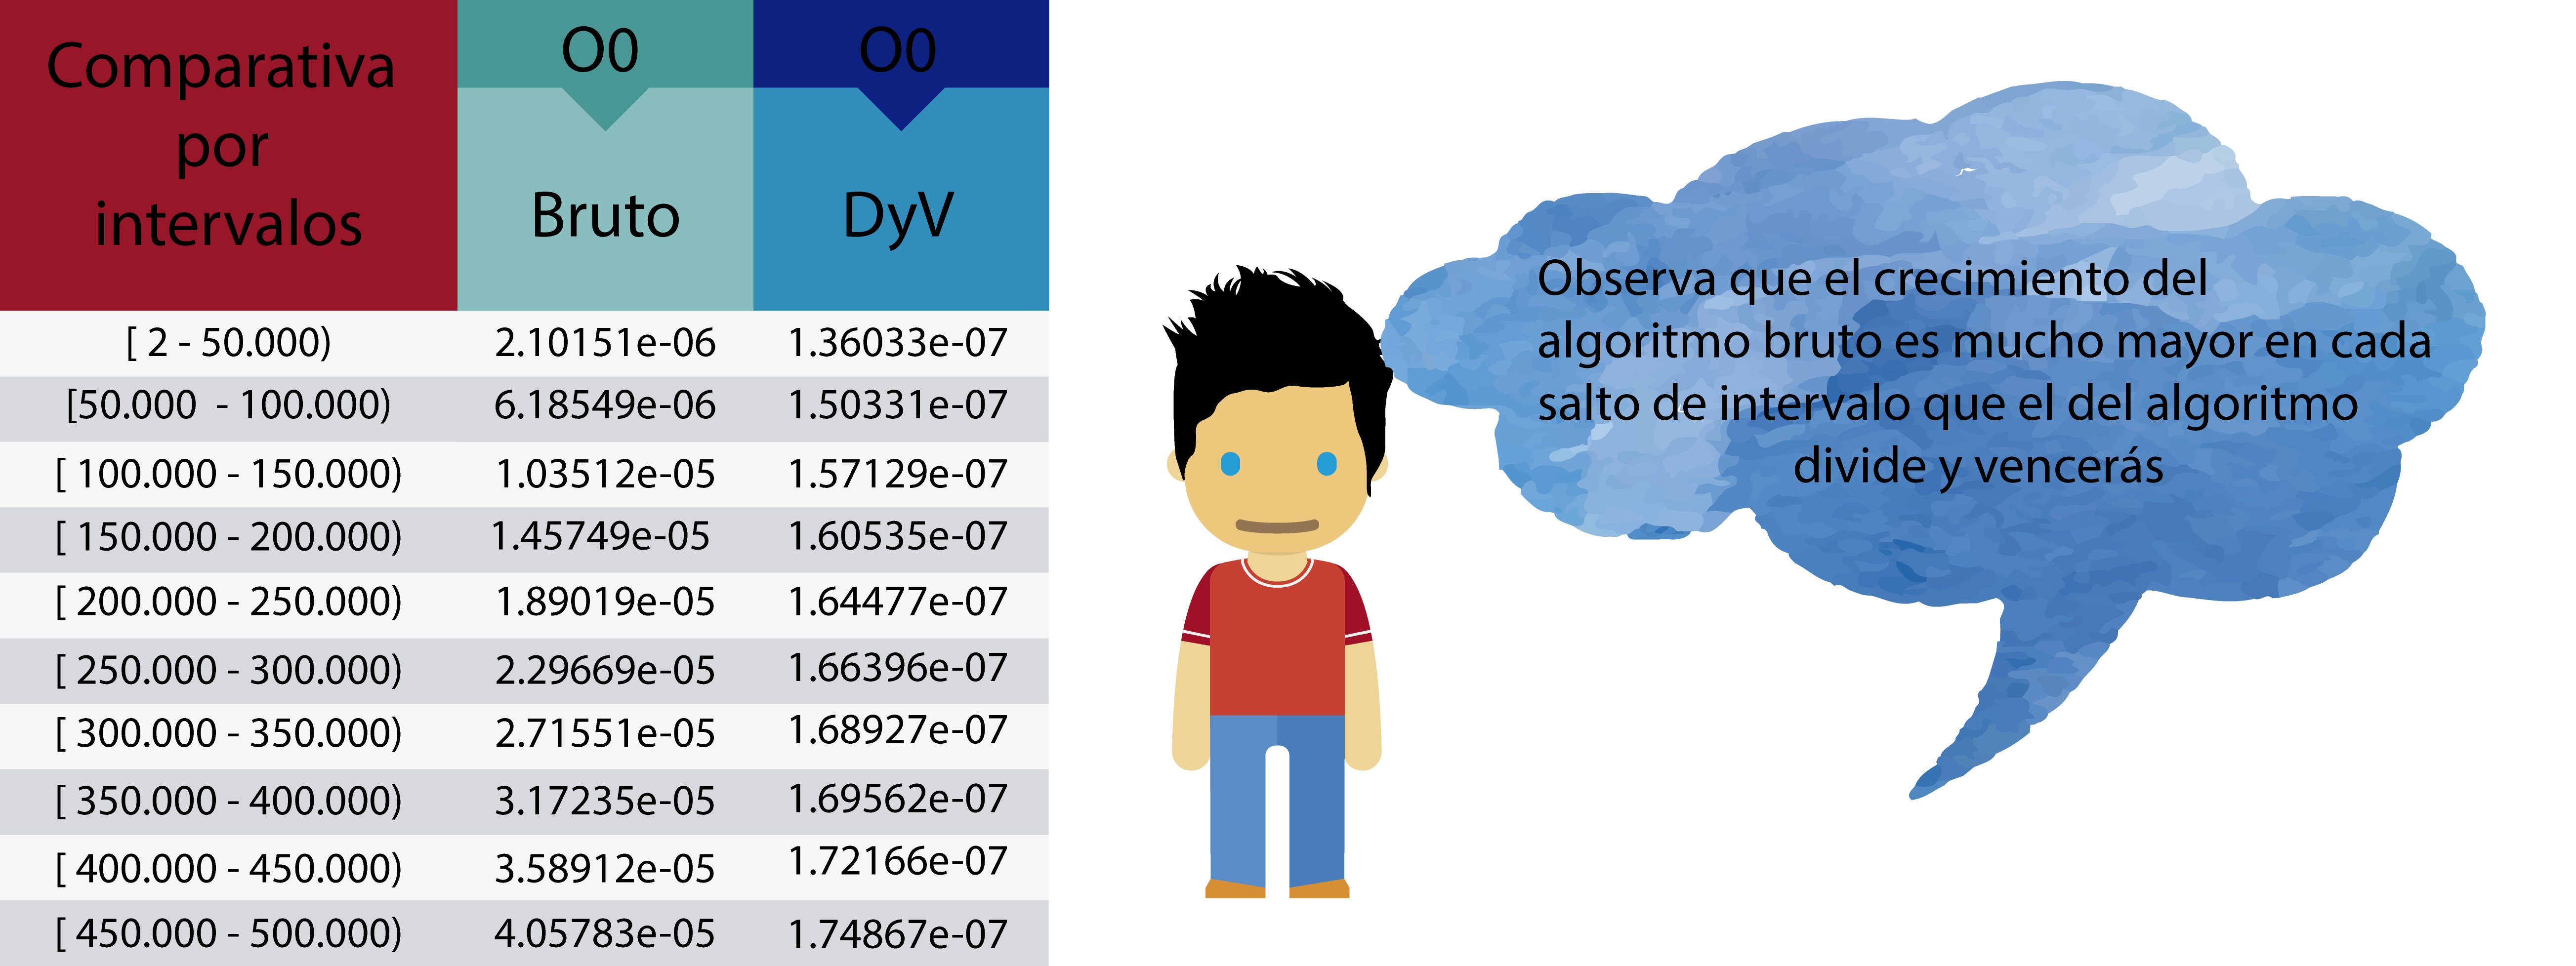
\includegraphics[width=12.0cm,height=5.3cm]{Images/TablaA-01}}
		\end{picture}
		\end{center}
		\end{figure}
		
	\end{frame}
	
	\begin{frame}[plain]
	\frametitle{Tabla Optimizacion 1}
		\begin{figure}[htb]
		\begin{center}
		\begin{picture}(160,0)
		\put(-80,-100){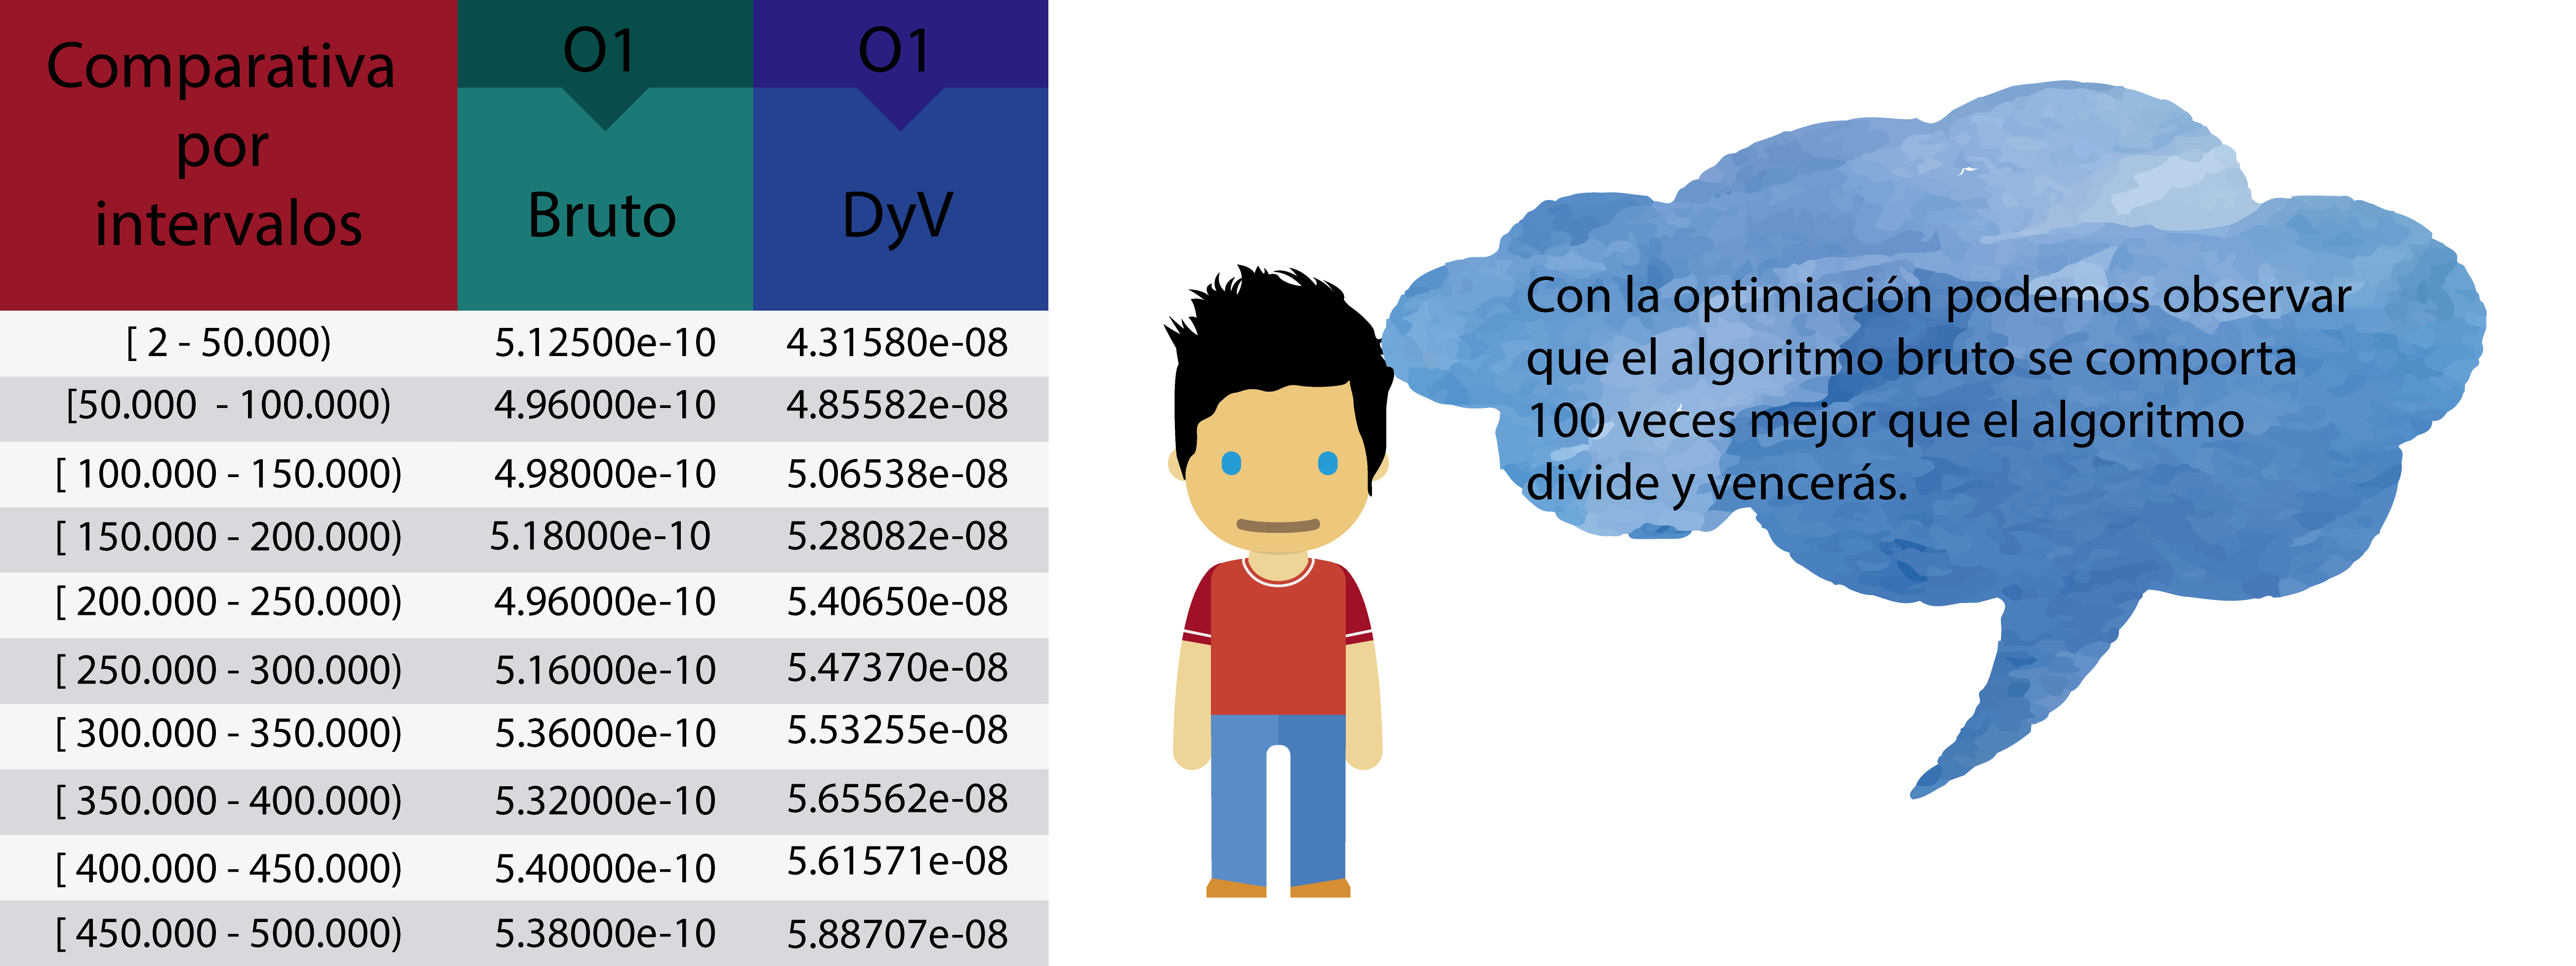
\includegraphics[width=12.0cm,height=5.3cm]{Images/TablaB-02}}
		\end{picture}
		\end{center}
		\end{figure}
		
	\end{frame}	
	
	
	
	\begin{frame}[plain]
	\frametitle{Tabla Optimizacion 2}
		\begin{figure}[htb]
		\begin{center}
		\begin{picture}(160,0)
		\put(-80,-100){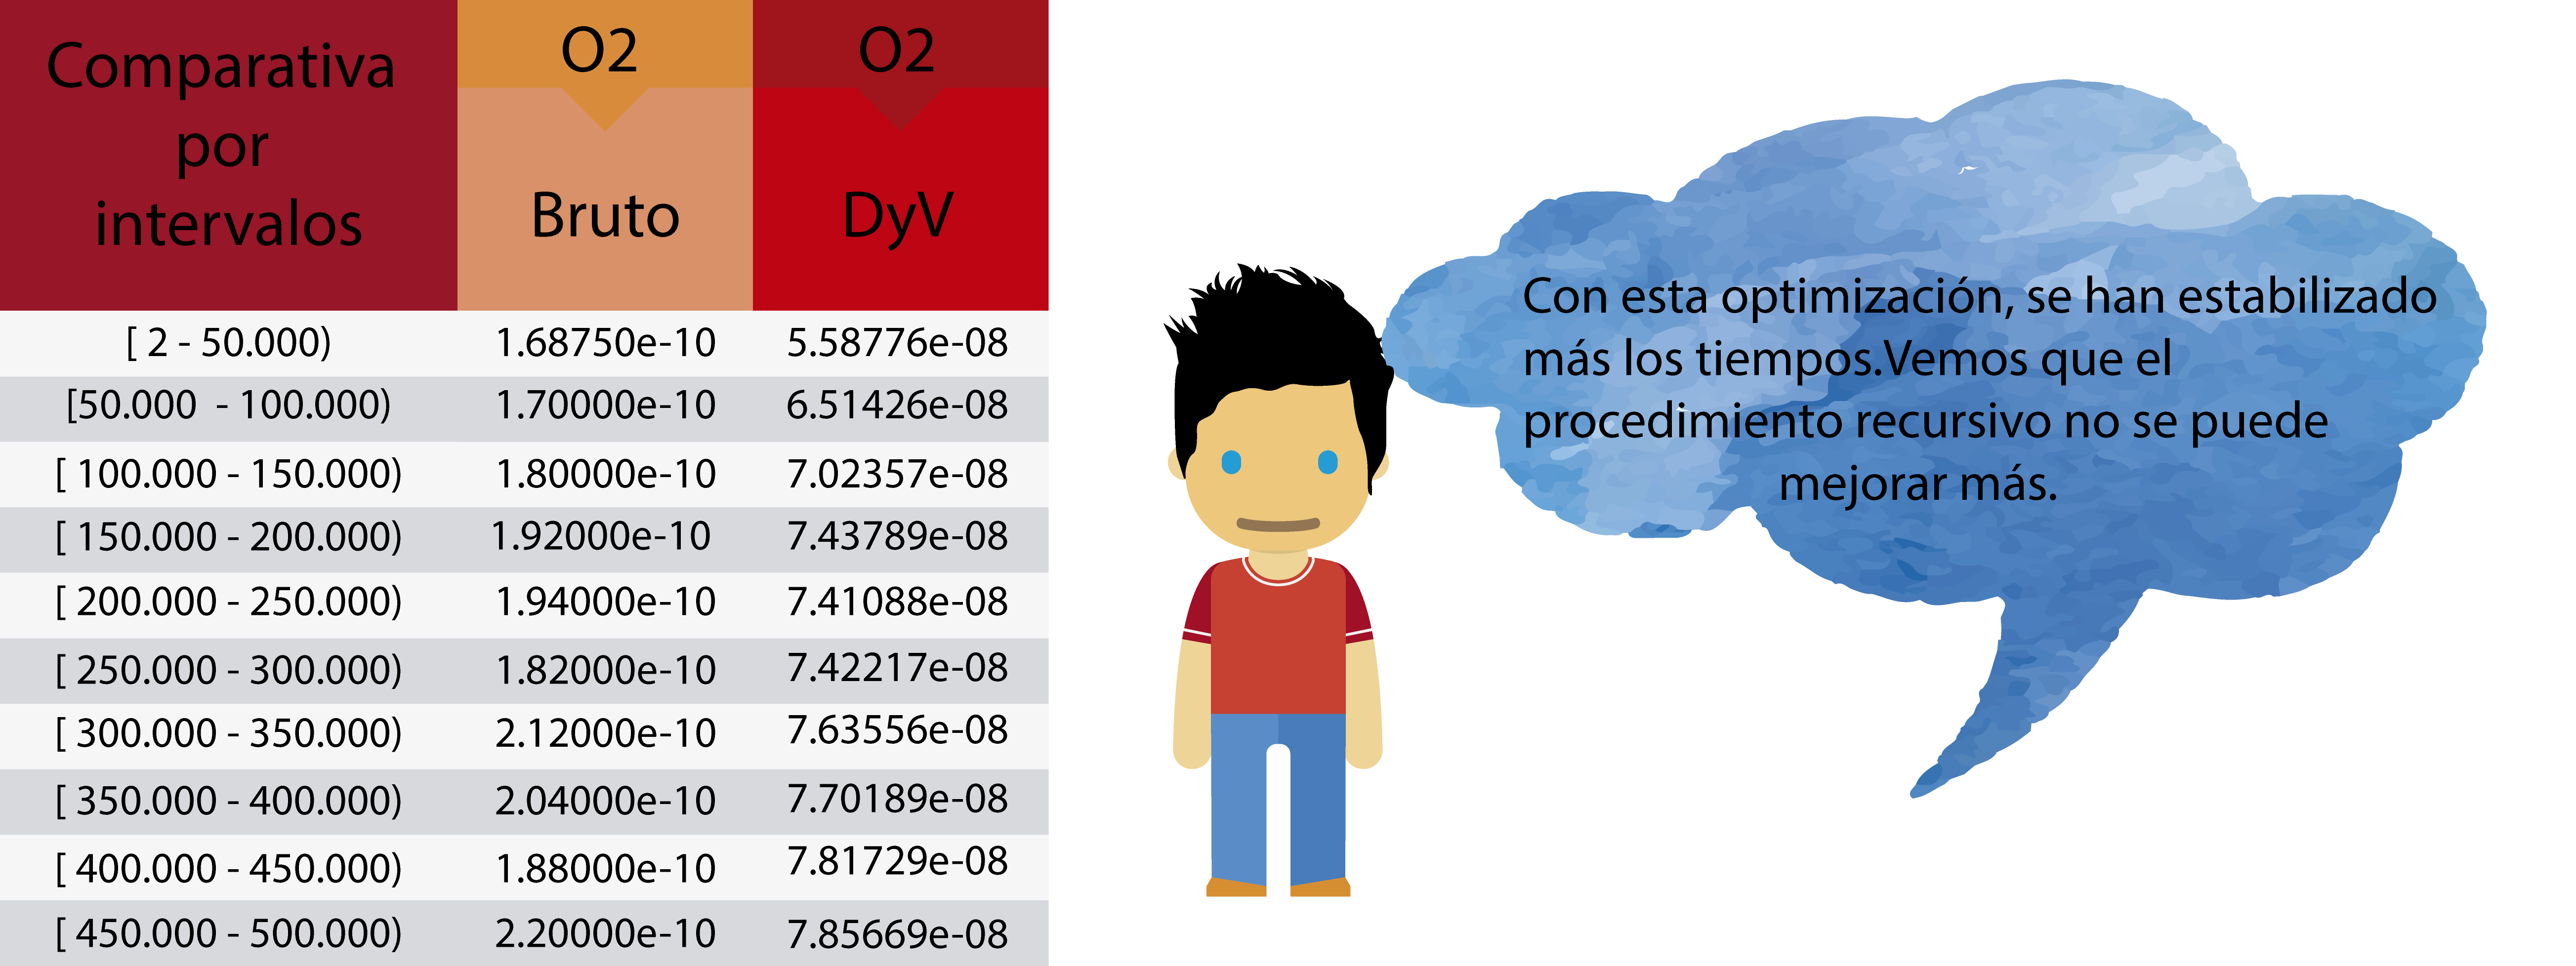
\includegraphics[width=12.0cm,height=5.3cm]{Images/TablaC-03}}
		\end{picture}
		\end{center}
		\end{figure}
		
	\end{frame}		


	\begin{frame}[plain]
	\frametitle{Tabla resumen}
		\begin{figure}[htb]
		\begin{center}
		\begin{picture}(160,0)
		\put(-95,-110){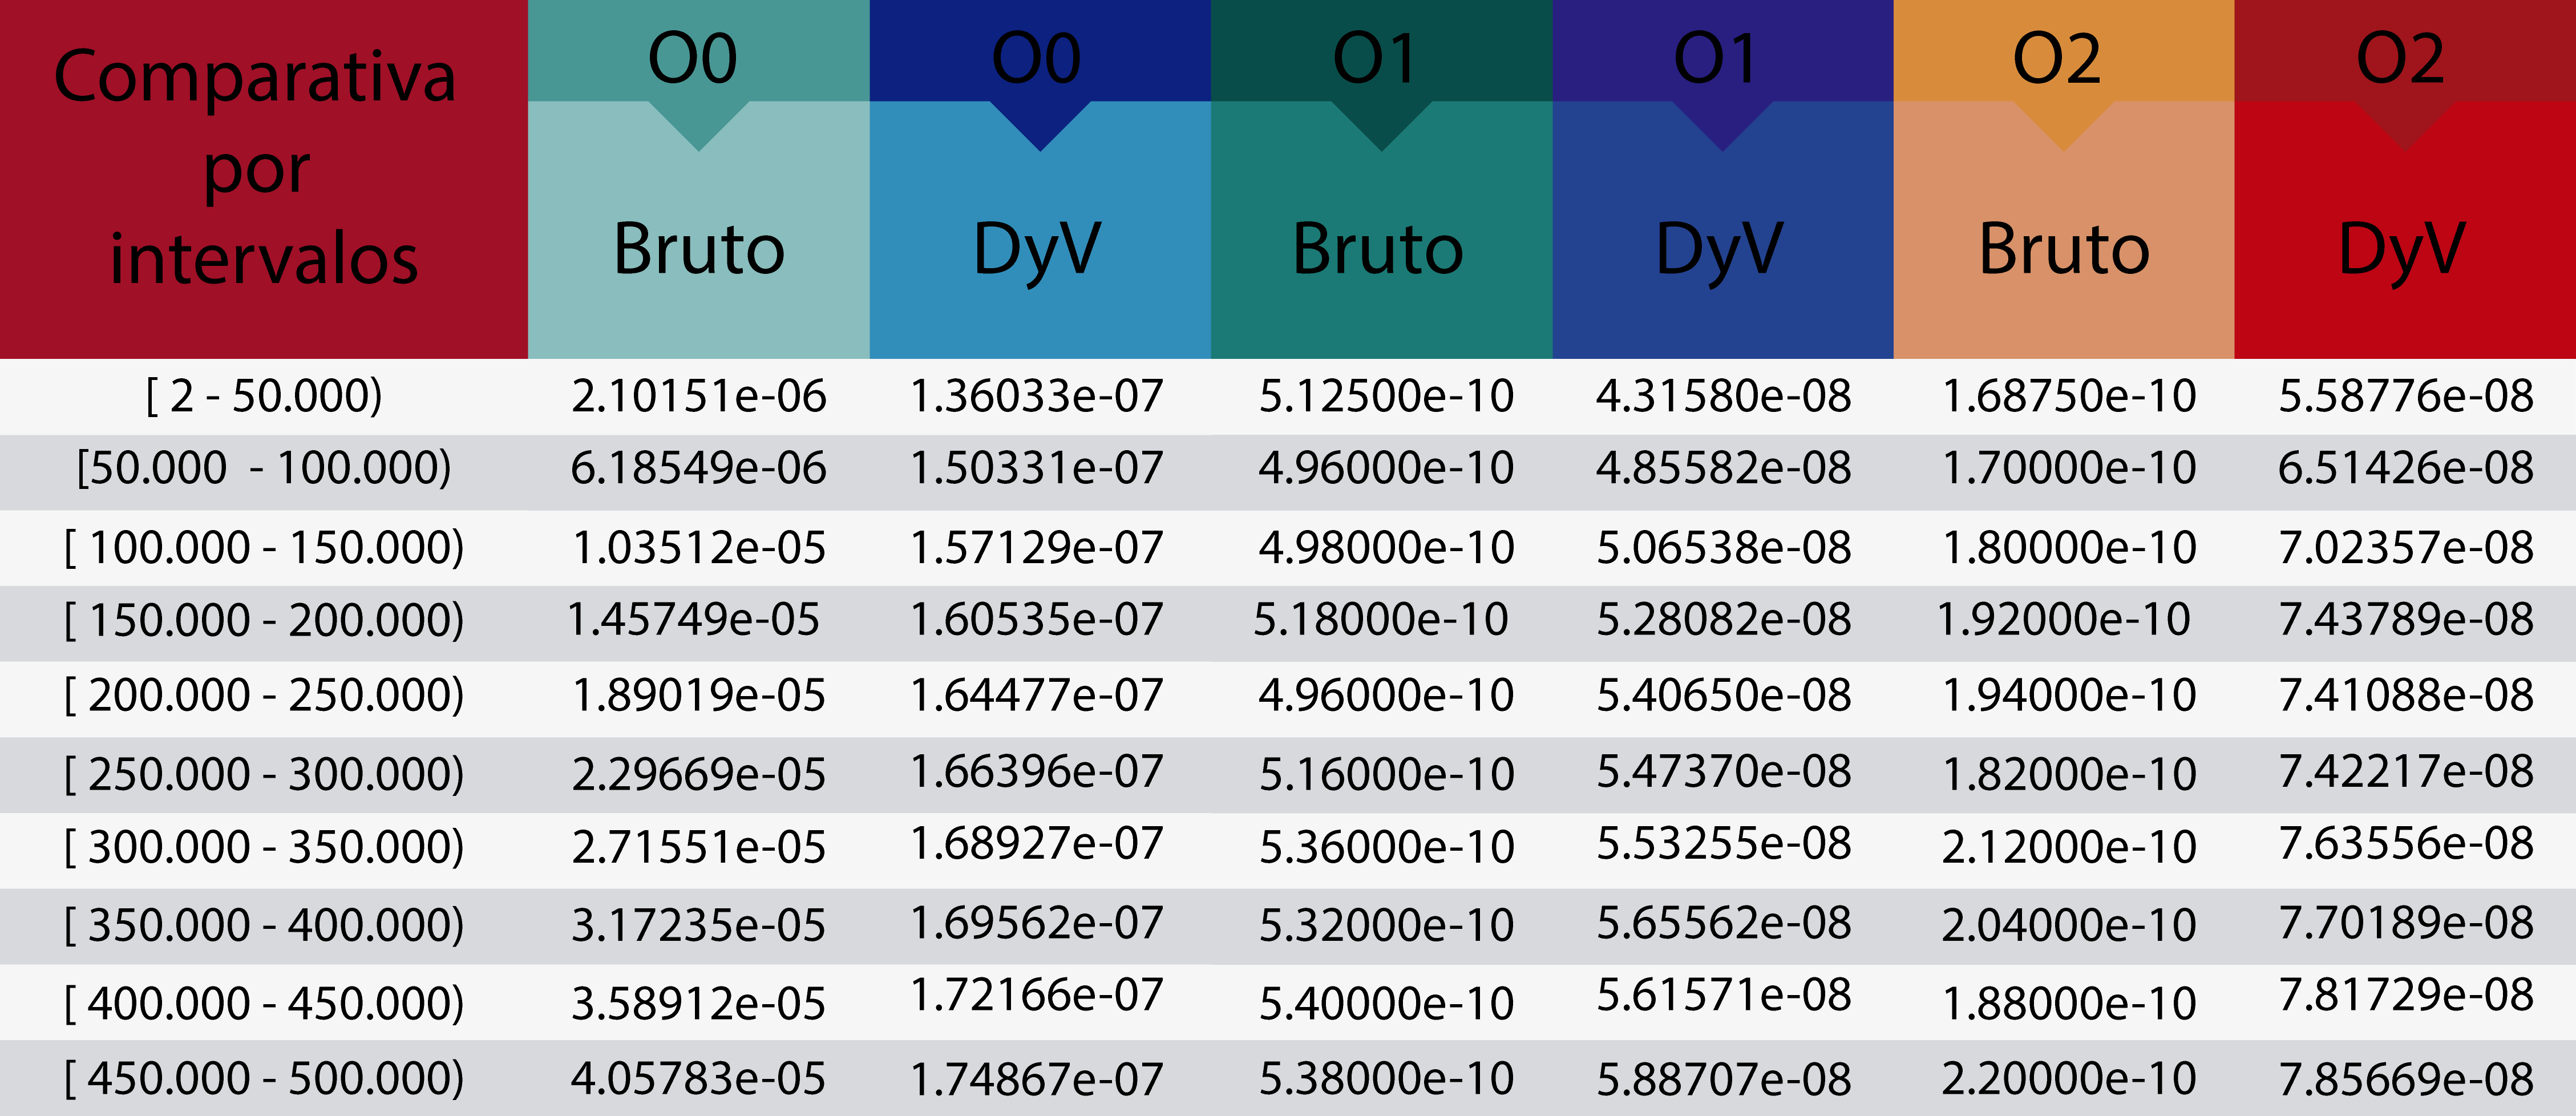
\includegraphics[width=12.1cm,height=6.9cm]{Images/TablaD-04}}
		\end{picture}
		\end{center}
		\end{figure}
		
	\end{frame}	
	
	\begin{frame}[plain]
	\frametitle{Agradecimientos}
		\begin{figure}[htb]
		\begin{center}
		\begin{picture}(160,0)
		\put(-110,-180){
\includegraphics[width=13.5cm,height=8.7cm]{Images/TablaAgradecimiento-05}}
		\end{picture}
		\end{center}
		\end{figure}
		
	\end{frame}	
	
	
	
	
	


	
	
	
	
	

	
	
	